\section{Ocenjevanje uspešnosti klasifikacijskih tehnik}

Ločujemo med merami uspešnosti klasifikacijskih tehnik in pristopi, kako te mere ocenimo. Pri slednjih je nadvse pomembno, da uspešnost nikoli ne ocenjujemo na učnih primerih. Ocenjevanje uspešnost mora biti izvedeno le na primerih, ki jih v postopku izdelave napovednega modela ali v kateremkoli njegovem delu nismo uporabili oziroma videli.

\subsection{Postopki ocenjevanja uspešnosti}

Iz osnovne, celotne množice z razredom označenih primerov $D$ izberimo vzorec učnih primerov $D_L$ in testnih primerov $D_T$, tako da, tipično, $D_L\cap D_T=\emptyset$ in $D_L\cup D_T=D$. Učne primere uporabimo za razvoj napovednega modela, katerega točnost nato preskusimo na testnih primerih. Da ocena točnosti ni odvisna od ene same delitve množice primerov, postopek večkrat ponovimo in poročamo o povprečni statistiki oziroma meri, ki smo jo uporabili za ocenjevanje algoritmov uvrščanja. Tehnike, ki jih pri tem lahko uporabimo, so:
\begin{description}
\item[Prečno preverjanje] reda $k$ \angl{k-fold cross validation}, kjer množico vseh primerov razdelimo na $k$ enakih množic in od teh pri vsakem od $k$ korakov eno uporabimo za testiranje, vse ostale pa za učenje.
\item[Izloči enega] \angl{leave-one-out}, pri čemer iz množice primerov vsakič izločimo en sam primer, na katerem bomo zgrajeni napovedni model testirali, vse ostale primere pa uporabimo za gradnjo modela. Postopek je predvsem primeren za manjše nabore podatkov.
\item[Metoda stremena] \angl{bootstrap} kjer iz množice z $N$ primeri z vračanjem naključno izberemo enako veliko množico za učenje in vse neizbrane primere uporabimo za testiranje. Vzorčenje, gradnjo modela in testiranje večkrat ponovimo. Tipično je takih ponovitev sto ali nekaj sto, tudi do tisoč.
\end{description}

\subsection{Mere}

\begin{table}[htbp]
\caption{Kontingenčna tabela ali tabela napak \angl{confusion matrix}.}
\label{t-confusion-matrix}
\begin{center}
\begin{tabular}{rcccc}
& & \multicolumn{2}{c}{Dejanska vrednost} \\ 
& & $+$ & $-$ \\
\cmidrule(r){3-4}
Napovedana & $+$ & True Positive ($TP$) & False Positive ($FP$) & $P'$ \\
vrednost & $-$ & False Negative ($FN$) & True Negative ($TN$) & $N'$ \\ \cmidrule(r){3-4}
& & $P$ & $N$ \\
\end{tabular}
\end{center}
\end{table}

\begin{description}
\item[zadetek] (TP), \angl{true positive}
\item[pravilna zavrnitev](TN), \angl{true negative}
\item[napačno pozitiven, lažni alarm] (FP), napaka I. reda \angl{false positive}
\item[pogrešek] (FN), napaka II. reda \angl{false negative}
\item[občutljivost, priklic] \angl{sensitivity, true positive rate, recall}, $TPR = {TP / P} = {TP / (TP+FN)} $
\item[delež napačno pozitivnih], odpadek (FPR), \angl{false positive rate, fall-out} $FPR = FP / N = FP / (FP + TN)$
\item[točnost] (ACC), \angl{accuracy}, $ACC = (TP + TN) / (P + N)$
\item[specifičnost], stopnja pravilne zavrnitve (SPC), \angl{specificity, true negative rate}, $SPC = TN / N = TN / (FP + TN) = 1 - FPR$
\item[natančnost], delež pravilnih pozitivnih (PPV), \angl{positive predictive value, precision} $PPV = TP / (TP + FP)$
\item[delež pravilnih negativnih] (NPV), \angl{negative predictive value}, $NPV = TN / (TN + FN)$
\item[mera F1] (F1) \angl{F1 score}, $F1 = 2TP^2/(P+P')$
\end{description}

\subsection{Površina pod krivuljo ROC}

Prav posebna mera je površina pod krivuljo ROC \angl{area under Receiving Operator Characteristics curve} in zato zasluži poseben razdelek. Mero so najprej uporabili v ameriški vojski tekom druge svetovne vojne in z njo skušali oceniti radariste ter njihovo točnost pri razlikovanju med zavezniškimi in agresorjevimi letali na radarskem zaslonu. Ocenjevali so jih v različnih pogojih (dopoldne, zvečer, po neprespani noči, ...) in ob različnih časih ter skušali, ne glede na njihovo stanje, radariste kar najbolj objektivno rangirati, od teh zelo uspešnih do drugih, ki so bolj često delali napake. Mero so ponovno odkrili v 1970-ih in jo najprej uporabljali v radiologiji, kasneje pa na celotnem področju medicine. Da bi jo potem znova odkrili na prelomu stoletja in pričeli množično uporabljati na celotnem področju statistike in odkrivanja znanj iz podatkov.

Oglejmo si najprej konstrukcijo krivulje ROC na primeru. Denimo, da smo že zgradili model uvrščanja in bi radi ocenili njegovo točnost na testnih primerih. Naš klasifikacijski problem je dvovrednostni, napovedni model pa zna napovedati verjetnosti ciljnega razreda $p(+|X)$, kjer je $X$ atributno opisan primer.

\begin{table}[htbp]
\caption{Testni primeri z dejanskim razredom in verjetnostjo razred ``yes'', kot jo je predlagal napovedni model, katerega točnost ocenjujemo. Primeri so urejeni skladno z napovedano verjetnostjo.}
\label{t-auc}
\begin{center}
\begin{tabular}{cc}
\toprule
Razred & $p(+|X)$ \\
\midrule
+ & 0.89 \\
+ & 0.80 \\
+ & 0.80 \\
- & 0.80 \\
+ & 0.63 \\
- & 0.33 \\
+ & 0.33 \\
- & 0.10 \\
- & 0.10 \\
- & 0.10 \\
\bottomrule
\end{tabular}
\end{center}
\end{table}

Točnost uvrščanja primerov s tabele~\ref{t-auc} je odvisna od praga verjetnosti $p_T$, nad katerimi bomo razglasili, da primeri pripadajo pozitivnemu razredu. Pri tem bomo opazovali $TPR$, to je delež pravilno napovedanih pozitivnih primerov med vsemi dejansko pozitivnimi \angl{true positive rate}, in $FPR$, delež negativnih primerov, za katere je bila napoved napačna \angl{false positive rate}. Izrazimo ti dve meri še z notacijo iz prejšnjega razdelka:
$$ TPR = {TP \over P} $$
$$ FPR = {FP \over N} $$

Vzemimo, da vse primere razglasimo kot pozitivne ($p_T<0.10$). Na ta način smo pravilno ``ulovili'' vse dejansko pozitivne primere in s tem dosegli najvišji delež pravilno napovedanih pozitivnih primerov med vsemi dejansko pozitivni primeri ($TP=P$, $TPR=1.0$). Tudi $FPR$ je s tem maksimalni, 1.0, saj smo vse negativne primere napačno uvrstili med pozitivne.

Drugače pa je, če vse primere iz testne razglasimo kot negativne ($p_T>0.89$). Primerov, ki bi jih razglasili za pozitivne, ni, zato $TPR=0$ in $FPR=0$.

Vse ostale vrednosti $TPR$ in $FPR$ bodo, za prag, ki ga izberemo med zgornjima dvema skrajnima mejama, nekje med 0 in 1. Najbolj zaželen prag bi bil tam, kjer bi vse razvrstitve v pozitivni razred bile pravilne in nobena ne bi bila nepravilna. V tej točki bi bil $TPR=1$ in $FPR=0$. Ali za naš primer taka vrednost praga obstaja?

Preskusimo sedaj vse možne mejne vrednosti $p_T$, kjer bi se nam vrednosti $TPR$ in $FPR$ lahko spremenile. Za naše podatke imamo štiri intervale, kjer lahko poiščemo take meje. Med 0.89 in 0.80, med 0.80 in 0.63, med 0.63 in 0.33, in med 0.33 in 0.10. Kje v teh intervalih bo dejansko naša mejna vrednost ni pomembno. Za te štiri meje izračunajmo sedaj vrednosti $TPR$ in $FPR$ in te vnesimo v graf (slika~\ref{f-roc}).

\begin{figure}[htbp]
\begin{center}
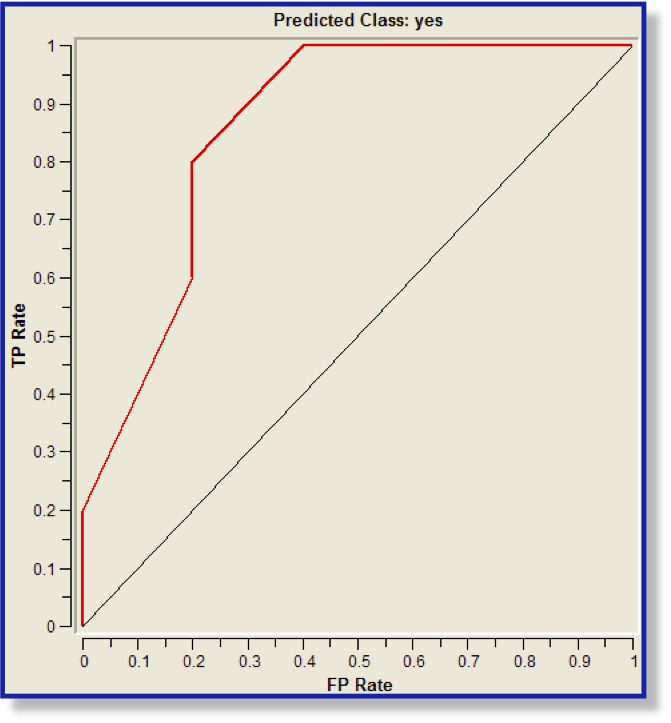
\includegraphics[width=7cm]{slike/roc.png}
\caption{Krivulja ROC za podatke s tabele~\ref{t-auc}.}
\label{f-roc}
\end{center}
\end{figure}

Obstaja tudi hitrejši način izrisa krivulja $ROC$, ki zahteva ureditev primerov po napovedani verjetnosti ciljnega razreda (kot smo to storili v tabeli~\ref{t-auc}). Postopek je naslednji:
%
\begin{enumerate}
\item Izrišemo graf z mrežo $1/N$ horizontalno in $1/P$ vertikalno.
\item Uredimo primere v seznam $L$ po padajoči verjetnosti napovedi v ciljni razred.
\item Pričnimo v točki (0,0).
\item Izberimo in iz seznama $L$ izključimo primere z najvišjo napovedano verjetnostjo. Naj ti primeri vključujejo $n_+$ primerov iz pozitivnega razreda, in $n_-$ primerov iz negativnega razreda. V mreži grafa se premaknimo $n_+$ razdelkov desno in $n_-$ razdelkov navzgor.
\item Če $L$ ni prazen, skoči na korak 4, sicer končaj.
\end{enumerate}

\begin{figure}[htbp]
\begin{center}
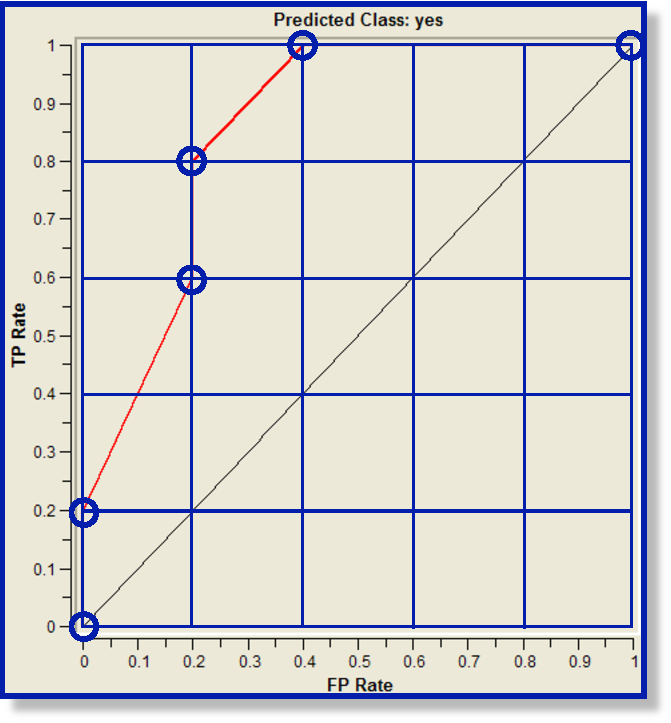
\includegraphics[width=7cm]{slike/roc-walk.pdf}
\caption{Mreža za izris krivulje ROC in sprehod po njenih točkah skladno s primeri s tabele~\ref{t-auc}.}
\label{f-roc-walk}
\end{center}
\end{figure}

Opazimo, da zgoraj opisan algoritem pravilno razpozna obe meri $TPR$ in $FPR$ za vse možne vrednosti praga verjetnosti (slika~\ref{f-roc-walk}).

Površino pod krivuljo ROC označimo z $AUC$. Pri naključnih napovedih pričakujemo, da bodo v obhodu zgornjega algoritma šli približno po diagonali grafi in bo $AUC=0.5$. To je tudi spodnja meja za to mero in je karakteristična za neuspešen napovedni model. Dejansko je meja za uspešne modele tipično pri $AUC=0.75$, modeli, ki imajo visoko napovedno točnost, pa imajo $AUC$ nekje nad $0.9$.

Površina pod ROC krivuljo pa ima še eno zanimivo lastnost. Če opazujemo sprehod po mreži za izris ROC krivulje, opazimo, da površina pod vsakem segmentom ravno ustreza številu napačno razvrščenih primerov, katerih verjetnost pozitivnega razreda je nad določeno mejo. $AUC$ ustreza verjetnosti, da za naključno izbrani primer $X^+$ iz pozitivnega razreda in naključno izbrani primer $X^-$ iz negativnega razreda velja $p(+,X^+) > p(+, X^-)$.
